\section{\system{}\ Design}

\subsection{System Overview}

Figure~\ref{fig:architecture} shows the closed-loop, multi-fidelity Pareto
search and maps the requirements in Section~2 to concrete mechanisms.  The
Scenario Compiler enforces scenario conditioning (R1) by combining a typed
JSON/YAML specification with a natural-language intent and rejecting
infeasible candidates.  The evidence model and L0--L4 contracts preserve cross-scale
uncertainty (R2).  \ipig{}\ allocates measurement cost to decision-relevant
ambiguity (R3), while the guarded planner and Verifier bound semantic autonomy
(R4).  A language-model planner
observes the intent, a compact belief summary, remaining budget, failures, and
provenance, then emits one structured subgoal from \{\textsc{Explore},
\textsc{ResolveSLO}, \textsc{CalibrateScale}, \textsc{Repair}\}.  Final
\textsc{Verify} is entered only by the deterministic controller.  Within a
guarded search subgoal, \ipig{}\ selects the numerical
configuration--fidelity action.  The Tool Layer invokes serving simulation,
\bench{}\ templates, telemetry readers, and the scheduler.  Observations update
the Energy Twin and a versioned Evidence Store; the Verifier reruns final
Pareto candidates before scripts and recommendations are released.

\begin{figure*}[t]
\centering
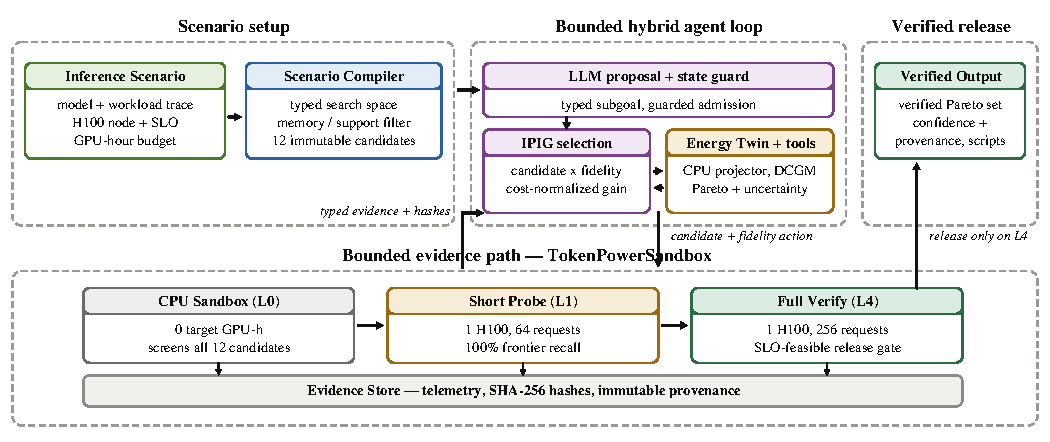
\includegraphics[width=\textwidth]{figures/results/fig2_system_overview.pdf}
\caption{\system{} overview.  The scenario compiler freezes a typed candidate
set and feasibility constraints.  The language model proposes an experiment
subgoal, the state guard admits or repairs it, and \ipig{} selects a
candidate--fidelity action.  The Energy Twin and deterministic tools produce
CPU predictions or measured H100 evidence, update uncertainty and the Pareto
set, and append telemetry and hashes to the evidence store.  Only full
target-workload Verify evidence can authorize the final recommendation.}
\label{fig:architecture}
\end{figure*}


\bench{}\ and \system{}\ consequently have separate responsibilities.  \bench{}\
defines and executes a measurement; \system{}\ decides which measurements are
decision-relevant, what can be inferred between them, and whether the evidence
supports a recommendation.  This separation also prevents circular claims:
the same simulator is never treated as ground truth for its own accuracy.

\subsection{Calibrated Energy Twin}

The implemented Energy Twin starts from a measured serving anchor and an
interpretable CPU projector.  It rejects memory-infeasible candidates, scales
prefill and decode work using token geometry and batch occupancy, predicts
active power between measured idle and active bounds, and preserves the
physical identity
\begin{equation}
\widehat E(W,x)=\widehat P(W,x)\widehat t(W,x).
\label{eq:energy-identity}
\end{equation}
For the present single-H100 study, one anchor cannot capture utilization
transitions across context length $L$ and concurrency $k$.  Relative to anchor
$(L_0,k_0)$, we therefore define
\begin{align}
q&=\log_2\!\frac{L_{in}+0.5L_{out}}{L_{in,0}+0.5L_{out,0}}, &
r&=\log_2\!\frac{k}{k_0},\\[-3pt]
\phi&=[q,r,qr,r^2].&&
\end{align}
For each directly predicted metric $m$, ridge regression fits
$\log(y_m/\widehat y_m^{base})=\beta_m^T\phi$.  Its strength is selected by
leave-one-workload-out error on a development split.  Throughput, power, TTFT,
and TPOT are corrected; energy is recomputed from corrected power and duration
rather than independently fitted.  Every calibration point retains repeat
dispersion and source hashes.

The topology projector additionally contains explicit TP/PP placement,
communication-volume, memory, and scale-distance terms.  At present these
terms produce machine-labeled extrapolations with enlarged uncertainty; they
are not publication-eligible multi-node predictions.  L2--L4 calibration on
H100/H200/B200 clusters is therefore an extension target rather than a claimed
result of this paper.

\subsection{Multi-Fidelity Sandbox Calibration}

The multi-fidelity sandbox is a bounded evidence environment implemented with
immutable job templates, container/runtime hashes, explicit resource
allocations, and fixed telemetry settings.  It does not pretend to reproduce a
large cluster on a laptop.  Instead, Figure~\ref{fig:calibration} organizes a
hierarchical set of evidence levels by the new effects they expose.

\begin{figure*}[t]
\centering
\begin{tikzpicture}[
  x=1cm,y=1cm,
  every node/.style={font=\sffamily},
  level/.style={draw=tpGray,rounded corners=2pt,minimum height=2.25cm,
    text width=2.55cm,align=center,inner sep=3pt,font=\scriptsize},
  flow/.style={-{Stealth[length=2.3mm]},line width=0.9pt,draw=tpGray}
]
  \node[level,fill=tpGrayLight] (l0) at (1.45,0.05)
    {\textbf{L0: Replay}\\[2pt]\textbf{0 GPUs}\\history retrieval\\analytic / event simulation\\\emph{simulated}};
  \node[level,fill=tpBlueLight] (l1) at (4.85,0.25)
    {\textbf{L1: Phase Probe}\\[2pt]\textbf{1 GPU}\\idle + warmup\\prefill / decode buckets\\\emph{device measured}};
  \node[level,fill=tpTealLight] (l2) at (8.25,0.45)
    {\textbf{L2: Node Probe}\\[2pt]\textbf{2--8 GPUs}\\TP / PP collectives\\NVLink / PCIe + KV\\\emph{node measured}};
  \node[level,fill=tpGoldLight] (l3) at (11.65,0.65)
    {\textbf{L3: Scale Probe}\\[2pt]\textbf{2+ nodes}\\fabric + placement\\sync / pipeline gaps\\\emph{sparse measured}};
  \node[level,fill=tpRoseLight] (l4) at (15.05,0.85)
    {\textbf{L4: Verification}\\[2pt]\textbf{target scale}\\arrival-trace replay\\queue + SLO behavior\\\emph{verified measured}};

  \draw[flow] (l0.east) -- (l1.west);
  \draw[flow] (l1.east) -- (l2.west);
  \draw[flow] (l2.east) -- (l3.west);
  \draw[flow] (l3.east) -- (l4.west);
  \draw[-{Stealth[length=2.5mm]},very thick,tpRose]
    (0.0,-1.55) -- node[below,font=\scriptsize\bfseries,text=tpRoseDark]
    {increasing fidelity, topology coverage, and GPU-hour cost} (16.65,-1.55);
\end{tikzpicture}
\caption{Multi-fidelity sandbox calibration.  Each hierarchical level exposes
effects that cannot be inferred reliably below it.  The agent escalates only
candidates whose uncertainty can change SLO feasibility or the Pareto frontier;
a final deployment recommendation requires target-scale trace verification.}
\label{fig:calibration}
\end{figure*}


\begin{itemize}
    \item \textbf{L0 -- replay/simulate (0 GPUs):} retrieve nearby \bench{}\
    records and run analytic or discrete-event simulation.
    \item \textbf{L1 -- phase probes (1 GPU):} measure idle/warmup, length- and
    batch-bucketed prefill, controlled decode, and power-policy response.
    \item \textbf{L2 -- intra-node probes (2--8 GPUs):} calibrate TP/PP,
    collective volume, NVLink/NVSwitch or PCIe behavior, and KV-cache pressure.
    \item \textbf{L3 -- sparse multi-node probes (2+ nodes):} sample selected
    scale points to expose fabric, synchronization, placement, and pipeline
    effects.  This level is deliberately sparse and chosen actively.
    \item \textbf{L4 -- target-trace verification:} replay the intended request
    trace for the top-$k$ configurations at target scale and report the result
    as measured evidence.
\end{itemize}

Levels are scenario-relative.  In the present single-H100 search, L1 is a
64-request probe and L4 is the full 256-request target workload on the same GPU;
L2 and L3 are skipped because the scenario contains no intra- or inter-node
scale transition.  A future multi-node scenario would activate those levels
without changing the controller or evidence schema.

A result carries its highest supporting level.  L0 outputs are
\emph{simulated}; predictions between observed settings are \emph{interpolated};
cross-topology predictions are \emph{extrapolated}; and only L1--L4 telemetry
is \emph{measured}.  This vocabulary is encoded in the artifact schema and
used in every table and plot.

\subsection{Hybrid Belief-State Policy and \ipig{}}

The controller observes predictive uncertainty, Pareto ambiguity, distance to
an SLO boundary, topology novelty, remaining budget, and run failures within
the loop in Figure~\ref{fig:architecture}.  It rejects invalid candidates
deterministically.  For each $x$, define high-fidelity feasibility and Pareto
membership variables $Q_x=\mathbf 1[q_S(x)=1]$ and
$P_x=\mathbf 1[x\in\mathcal P_S^*]$.  The intent-specific terminal decision is
\begin{equation}
\Omega_S=\{(Q_x,P_x):x\in\mathcal X_S\}.
\end{equation}
For an admissible action $a=(x,\ell)$, the policy interface targets
\begin{equation}
\alpha_t(a\mid S)=
\frac{I(Y_a;\Omega_S\mid\mathcal D_t,S)}
{(\mathbb E[c(a)\mid\mathcal D_t]+\epsilon)^\gamma}.
\label{eq:ipig}
\end{equation}
The numerator denotes information about the L4 SLO-feasible Pareto decision,
not generic prediction variance.  The current artifact exposes this estimator
as a typed interface and uses a transparent proxy
\begin{equation}
\widetilde I_t(a)=U_t(x)
\left(.45p_{P}(x)+.35p_{S}(x)+.20d_{T}(x)\right)g_\ell,
\label{eq:ipig-proxy}
\end{equation}
where $U_t$ is predictive uncertainty, $p_P$ approximates frontier relevance,
$p_S$ approximates proximity to an SLO boundary, $d_T$ flags unresolved
topology transfer, and $g_\ell$ is a monotone fidelity gain.  The semantic
subgoal increases the corresponding SLO or topology term.  The score divides
Eq.~\ref{eq:ipig-proxy} by declared GPU cost as in
Eq.~\ref{eq:ipig}; actions that exceed the remaining exploration budget are
removed first.  This proxy is auditable and sufficient for the Workshop
agent-loop study.  Replacing it with nested-posterior Pareto mutual information
is reserved for the larger MLSys evaluation.

The semantic subgoal restricts the admissible actions before maximizing
Eq.~\ref{eq:ipig}.  \textsc{ResolveSLO} admits candidates whose intervals
cross an SLO; \textsc{CalibrateScale} requires topology-sensitive features;
and the deterministic \textsc{Verify} state admits only L4 actions.
Operationally, the resulting
states are:
\begin{itemize}
    \item \textbf{Simulate} when the candidate is in-domain and its confidence
    interval cannot alter the feasible frontier.
    \item \textbf{Calibrate} when a local measurement can change ranking,
    reduce topology uncertainty, or resolve an SLO boundary.
    \item \textbf{Verify} when a candidate will be recommended, when scale
    extrapolation remains material, or when independent evidence is required.
\end{itemize}
Exploratory search terminates when its budget is exhausted or the probability
of a frontier change falls below a threshold.  A reserved verification budget
then supports L4 runs for the top-$k$ candidates; no recommendation is released
without target-scale evidence.

\subsection{Bounded Autonomy and Provenance}

The LLM can choose from typed tools but cannot issue an unrestricted shell
command, modify model weights, change telemetry intervals, or enlarge a Slurm
allocation without approval.  Numeric calculations, feasibility, Pareto
sorting, and budget accounting are deterministic.  Every action records the
scenario and configuration hashes, prompt and tool versions, evidence level,
job ID, raw-data URI, simulator checkpoint, uncertainty, and decision rationale.
The Verifier checks units, missing samples, clock/power state, run completion,
and agreement between GPU and node telemetry before accepting evidence.
